\documentclass[14pt,hyperref={CJKbookmarks=true}]{beamer}
\usepackage[space,noindent]{ctex}
\usepackage{amsmath}
\usepackage{graphics}
\usetheme{AnnArbor}
\setbeamercolor{normal text}{bg=black!10}
\begin{document}
\kaishu
\title[期中展示]{最小二乘法与正态分布}
\subtitle[期中展示]{从误差谈起}
\institute[生命科学学院]{南京大学\ 生命科学学院}
\begin{frame}
\titlepage
\end{frame}
\section{引入}
\subsection{统计学?}
\begin{frame}
\begin{quote}
There are three kinds of lies: lies, damned lies,
and statistics.
\end{quote}
\end{frame}
\subsection{数学王子——高斯}
\begin{frame}
卡尔·弗里德里希·高斯(Carl Friedrich Gauß)
\begin{itemize}
\item 数学家、物理学家、天文学家
\item 有“数学王子”之称
\item 以“高斯”命名的成果达110个
\end{itemize}
\end{frame}
\subsection{谷神星(Ceres)}
\begin{frame}
\begin{itemize}
\item 1766年,约翰·提丢斯(Johann Daniel Titius)发现行星到太阳距的距离比例有一定联系
\item 1801年1月,朱塞普·皮亚齐(Giuseppe Piazzi)观测到一颗“星星”
\item 同年,朱塞普·皮亚齐病倒,痊愈后“星星”已无法找到
\end{itemize}
\begin{theorem}{提丢斯-波得定则}
假设地球与太阳的距离为1,行星离太阳距离 $d = 0.4 + 0.3*2^{n-2}$ ,$n$为行星的序号。
\end{theorem}
\end{frame}
\begin{frame}
\begin{itemize}
\item 1801年9月,天文学家的争执引起高斯的注意,并决定通过计算找出
\item 1801年12月,高斯宣布计算出行星位置,并得到观测实验的证实
\item 1809年,高斯在其著作《天体运动论》中公布方法——最小二乘法(Least squares method)
\end{itemize}
\end{frame}
\section{最小二乘法}
\begin{frame}{最小二乘法}
\begin{itemize}
\item 误差的判据:观测值与理论值差的平方和
\item 目标:找出最匹配的曲线$y=\beta_{1}+\beta_{2}x$
\item 理想曲线:使所有观察值的残差平方和达到最小
\end{itemize}
\end{frame}
\begin{frame}
\begin{itemize}
\item 高斯认为
\begin{itemize}
\item 回归分析的最小二乘法是最优的
\end{itemize}
\item 高斯希望找到满足最小二乘法的误差密度函数
\end{itemize}
\begin{theorem}{Gauss-Markov定理}
在给定经典线性回归的假定下,最小二乘估计量是具有最小方差的线性无偏估计量.
\end{theorem}
\end{frame}
\section{正态分布}
\subsection{高斯的假设}
\begin{frame}[fragile]
设真实值为$\theta$,$x_1,x_2,...,x_n$为n次相互独立的测量值,每次测量的误差为$e_i$,假设误差的密度函数为$f(e)$,则测量值的联合概率为n个误差的联合概率,为
\[L(\theta)=L(\theta;x_1,x_2,...,x_n)=\prod_{i=1}^{n}f(e_i)=\prod_{i=1}^{n}f(x_i-\theta)\]
高斯认为取$L(\theta)$最大值可作为$\theta$的估计值,即
%\[\overset{^}{\theta}=\text{arg}\underset{\theta}{\text{max}}=L(\theta)\] 
$L(\theta)$称为样本的似然函数,得到的估计值称为极大似然估计
\end{frame}
\begin{frame}
\begin{itemize}
\item 高斯猜测:极大似然估计$=$算术平均值
\begin{itemize}
\item 千百年来大家都认为算术平均是一个好的估计,那极大似然估计导出的就应该是算术平均!
\end{itemize}
\end{itemize}
\end{frame}
\subsection{高斯的推导}
\begin{frame}
求极大似然估计,令
\[\frac{d\ln L(\theta)}{d\theta}=\frac{d}{d\theta}\sum_{i=1}^{n}\ln f(x_i-\theta)=0\]
\end{frame}
\begin{frame}[fragile]
整理得
\[\sum^{n}_{i=1}\frac{f'(x_i-\theta)}{f(x_i-\theta}=0\]
使用$g(x)=\frac{f'(x)}{f(x)}$替换,得到
\[\sum^{n}_{i=1}g(x_i-\theta)=0\]
假定$n=2$
\[g(x_1-\overline{x})+g(x_2-\overline{x})\]
且$x_1$,$x_2$任意,则有
\[g(-x)=-g(x)\]
\end{frame}
\begin{frame}[fragile]
再令$n=m+1$,且$x_1=x_2=\dots=x_m=-x$,$x_{m+1}=mx$
\[\sum^{n}_{i=1}g(x_i-\overline{x})=mg(-x)+g(mx)\]
\[\therefore g(mx)=mg(x)\]
唯一满足的连续函数:$g(x)=cx$ \newline
概率密度函数???
\end{frame}
\begin{frame}
对其积分,得:
\[\ln y = \frac{1}{2}cx^{2}+C\]
\[\Rightarrow f(x)=Me^{cx^{2}}\]
\end{frame}
\subsection{正态分布}
\begin{frame}{正态分布}
概率密度函数
\[f(x|\mu,\sigma)=\frac{1}{\sigma\sqrt{2\pi}}e^{-\frac{(x- \mu)^{2}}{2\sigma^{2}}}\]
对其进行标准化,使得$\mu=1$,$\sigma=1$
\[f(x)=\frac{1}{\sqrt{2\pi}}e^{-\frac{x^2}{2}}\]
\end{frame}
\begin{frame}
\begin{quote}
Many years ago I called the Laplace-Gaussian curve the normal curve, which name,while it avoids an international question of priority, has the disadvantage ofleading people to believe that all other distributions of frequency are in onesense or another "abnormal". \newline
-Karl Pearson (1920)
\end{quote}
\end{frame}
\begin{frame}
\begin{figure}
\centering
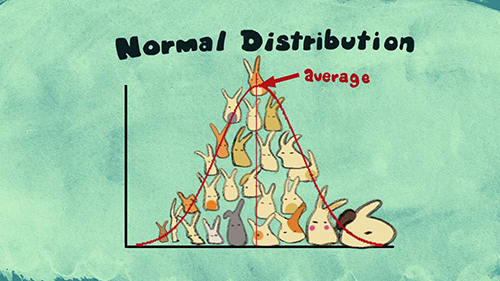
\includegraphics[scale=0.6]{Rabbits.jpg}
\end{figure}
\end{frame}
\subsection{中心极限定理}
\begin{frame}{中心极限定理}
\begin{theorem}
在适当的条件下,大量相互独立随机变量的均值经适当标准化后依分布收敛于正态分布
\end{theorem}
\begin{itemize}
\item 德莫佛-拉普拉斯定理
\begin{itemize}
\item 参数为$n,p$的二项分布以$np$为均值,$np(1-p)$为方差的正态分布为极限
\end{itemize}
\item 林德伯格-列维定理
\item 林德伯格-费勒定理
\end{itemize}
\end{frame}
\section{参考资料}
\begin{frame}
本次幻灯源码及演示
\begin{itemize}
\item https://github.com/Vladimir-Hu/
\end{itemize}
\end{frame}
\end{document}